\documentclass[12pt]{article}
\usepackage[utf8]{inputenc}
\usepackage[T1]{fontenc}
\usepackage{hyperref}
\usepackage[charter,expert]{mathdesign}
\usepackage[scaled=.96,osf]{XCharter}
\linespread{1.04}
\usepackage{geometry}
\usepackage{background}
\usepackage{float}
\usepackage{placeins}
\usepackage{tikz}
% workaround para redefining $ sign
% https://github.com/Wandmalfarbe/pandoc-latex-template/issues/184
\makeatletter
\global\let\tikz@ensure@dollar@catcode=\relax
\makeatother
\usepackage{lscape}
\usepackage{multicol}
\usepackage{amsmath}
\usepackage{pgfplots}
\usepackage{minted}

\usetikzlibrary{shapes.geometric, arrows, pgfplots.groupplots}
\pgfplotsset{compat=1.9}

\geometry{
	paper=a4paper,
	top=2.5cm,
	bottom=3cm,
	left=2.5cm,
	right=2.5cm,
	headheight=14pt,
	footskip=1.5cm,
	headsep=1.2cm
}

\backgroundsetup{
    position = {-3, -37},
    scale = 0.35,
    opacity = 1,
    angle = 90,
    contents = {
        
\includegraphics{logo.pdf}
    },
}

\renewcommand{\figurename}{Figura}

\tolerance=1
\emergencystretch=\maxdimen
\hyphenpenalty=10000
\hbadness=10000
\interfootnotelinepenalty=10000

\title{Tarea \#3\\ Herramientas HPC}
\author{Iñaki Amatria Barral\\ Alonso Rodríguez Iglesias}
\date{Noviembre 2021 -- Universidade da Coruña}

\begin{document}
\maketitle
\section{Introducción y objetivos}
En este documento se expone el proceso de análisis y optimización del código de la Tarea \#2 con el objetivo de conseguir un mejor tiempo de ejecución mediante la paralelización con OpenMP y siguiendo las recomendaciones de las herramientas ofrecidas por Intel oneAPI.
\section{Problemas de memoria}
En lo relativo a nuestra implementación, esta es muy sencilla y todos los \texttt{malloc} o \texttt{calloc} realizados tienen sus correspondientes \texttt{free} al final de la función. Sin embargo, el código original tiene memoria reservada, que al final de la ejecución, es \textit{still reachable}. En concreto, el programa termina sin liberar la memoria de \texttt{a}, \texttt{b}, \texttt{aref}, \texttt{bref}, \texttt{ipiv} e \texttt{ipiv2}. Esto no supone un gran problema, puesto que los recursos se liberan al finalizar el proceso, pero es una buena práctica el correcto manejo de la memoria.

Una vez solucionados estos detalles, se puede comprobar que no hay problemas de memoria mediante la ejecución de Valgrind (ver Figura \ref{fig:val}).

\begin{figure}
\centering
\begin{minted}[fontsize=\small, breaklines]{text}
==50130== Command: ./target/gnu/debug.out 24
==50130== 
Time taken by LAPACK: 0.10s
Time taken by my implementation: 0.00s
Result is ok!
==50130== 
==50130== HEAP SUMMARY:
==50130==     in use at exit: 0 bytes in 0 blocks
==50130==   total heap usage: 50 allocs, 50 frees, 98,736 bytes allocated
==50130== 
==50130== All heap blocks were freed -- no leaks are possible
==50130== 
==50130== For lists of detected and suppressed errors, rerun with: -s
==50130== ERROR SUMMARY: 0 errors from 0 contexts (suppressed: 0 from 0)
\end{minted}
\caption{Salida de Valgrind una vez solucionados los errores de memoria}
\label{fig:val}
\end{figure}
\section{Paralelización y vectorización}
Para la paralelización del código se ha seguido un enfoque incremental. De esta forma, se describe ahora el proceso seguido para paralelizar el código.

Como nuestro código no es, todavía, complejo, previo a la implementación se ha realizado un análisis en papel sobre los patrones de acceso a memoria de los diferentes bucles del código, así como un cálculo de la complejidad que estos representan. De esta forma, hemos podido entender mucho mejor como funciona nuestra implementación en términos de caché y, así, podemos entender mejor como paralelizar el código; evitando bloqueos innecesarios, por ejemplo.

Tras esta primera aproximación puramente teórica, se observan los \textit{hotspots} del código usando Intel VTune, que coinciden con los previstos. Esto es, los bucles \texttt{for} que realizan la descomposición LU, sustitución hacia delante y sustitución hacia atrás.

Después, se ha implementado una versión paralela del mismo mediante directivas de OpenMP, haciendo especial énfasis en dichos \textit{hotspots}, así como en el último bucle de transposición, donde la paralelización es trivial. Además, gracias al análisis en papel del código, se ha podido evitar sincronizaciones entre hilos innecesarias usando la directiva \texttt{nowait}.

Por último, y siguiendo los consejos de Intel Advisor y los reportes de optimización del Intel C Compiler, se han indicado los bucles sin dependencias (en este caso, todos) mediante el uso de \texttt{\#pragma ivdep}. Gracias a esta confirmación explícita por parte del programador, ICC (que no GCC) es capaz de vectorizar el código haciendo uso de las instrucciones AVX2, arrojando un \textit{Gain Estimate} de entre 2.15x y 3.64x (ver Figura \ref{fig:advisor_bucles}).
\section{Métricas del código}
La paralelización obtiene buenos rendimientos y la eficiencia de la paralelización es muy buena (ver Figura \ref{fig:metricas}). Sin embargo, exceptuando tamaños pequeños de matrices (menores a $n = 1024$), la implementación de LAPACK es mucho mejor, entre otros, porque nuestra implementación está \textit{memory-bound}, tal y como indica Intel VTune (ver Figura \ref{fig:micropipe}). La causa de esto está clara: la intensidad aritmética de nuestro algoritmo es muy baja. Es decir, tenemos un código que realiza operaciones sencillas (y muy rápidas) sobre datos que usa sólo una vez y, esto, acaba por saturar el bus y limitando la escalabilidad del código ---i.e. mal rendimiento---.
\section{Resultados}
Habiendo visto los resultados de ejecutar el código con Intel VTune, ya estamos en condiciones de interpretar las Figuras \ref{fig:speedups_o2} y \ref{fig:speedups_o3}, que muestran el \textit{speedup} de las funciones paralelas \texttt{my\_dgesv} con respecto a la implementación secuencial de \texttt{my\_dgesv} usando 1, 2, 4, 8 y 16 \textit{cores}\footnote{Los tiempos de ejecución y speedups, así como los logs de ejecución, se pueden encontrar en el la carpeta del proyecto, bajo la ruta \texttt{doc/resources}.}.

\begin{figure}[p]
    \centering
    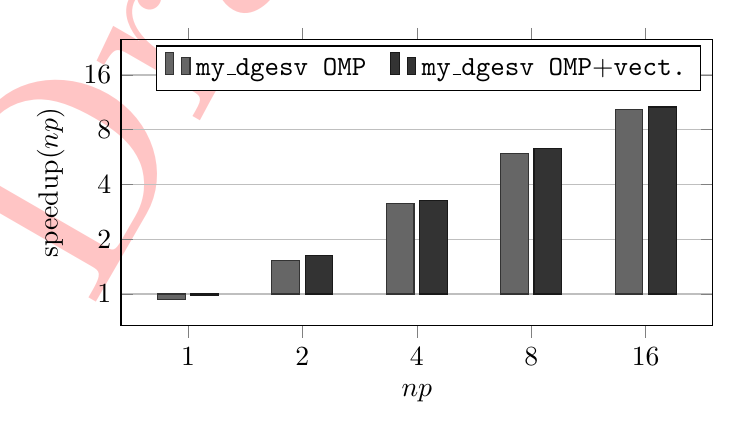
\begin{tikzpicture}
        \begin{axis}[ybar, width=0.75\linewidth, height=0.43\linewidth, xmode=log, ymode=log, log basis y={2}, log basis x={2}, enlarge x limits={abs=1.5}, xlabel={$np$}, ylabel={$\text{speedup}(np)$}, legend columns=2, ymin=0, ymax=25, ytick={1,2,4,8,16}, yticklabels={1,2,4,8,16}, xtick={1,2,4,8,16}, xticklabels={1,2,4,8,16}, ymajorgrids]
        \addplot[black!80, fill=black!60] coordinates {
            (1, 0.93)
            (2, 1.53)
            (4, 3.13)
            (8, 5.91)
            (16, 10.31)
        };
		\addplot[black!90, fill=black!80] coordinates {
            (1, 0.98)
            (2, 1.62)
            (4, 3.27)
            (8, 6.28)
            (16, 10.67)
        };
        \coordinate(d) at (0,22);% coordinate for the discontinuity
        \node[inner ysep=7pt,inner xsep=1.5pt,fill=white](D)at(d){};
        \draw(D.south west)--(D.north west) (D.south east)--(D.north east);
        \legend{\texttt{my\_dgesv OMP}\ \ \ , \texttt{my\_dgesv OMP$+$vect.}};
        \end{axis}
    \end{tikzpicture}
    \caption{\textit{Speedup} de \texttt{my\_dgesv} en el supercomputador FinisTerrae 2 con optimización O2 (ICC)}
    \label{fig:speedups_o2}
\end{figure}
\begin{figure}[p]
    \centering
    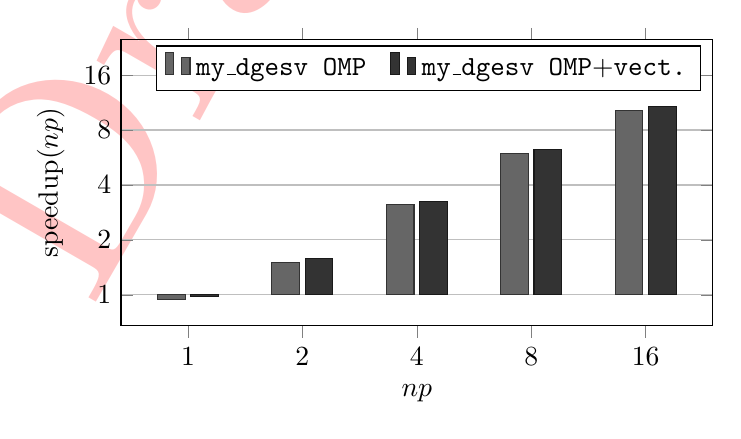
\begin{tikzpicture}
        \begin{axis}[ybar, width=0.75\linewidth, height=0.43\linewidth, xmode=log, ymode=log, log basis y={2}, log basis x={2}, enlarge x limits={abs=1.5}, xlabel={$np$}, ylabel={$\text{speedup}(np)$}, legend columns=2, ymin=0, ymax=25, ytick={1,2,4,8,16}, yticklabels={1,2,4,8,16}, xtick={1,2,4,8,16}, xticklabels={1,2,4,8,16}, ymajorgrids]
        \addplot[black!80, fill=black!60] coordinates {
            (1, 0.94)
            (2, 1.51)
            (4, 3.13)
            (8, 5.93)
            (16, 10.18)
        };
		\addplot[black!90, fill=black!80] coordinates {
            (1, 0.98)
            (2, 1.59)
            (4, 3.26)
            (8, 6.26)
            (16, 10.72)
        };
        \legend{\texttt{my\_dgesv OMP}\ \ \ , \texttt{my\_dgesv OMP$+$vect.}};
        \end{axis}
    \end{tikzpicture}
    \caption{\textit{Speedup} de \texttt{my\_dgesv} en el supercomputador FinisTerrae 2 con optimización O3 (ICC)}
    \label{fig:speedups_o3}
\end{figure}

Los resultados son sencillos de explicar. En general, como se pudo ver ya en la tarea anterior, compilar con O3 sobre O2 no ofrece prácticamente ningún tipo de mejora en tiempo de ejecución. Las aceleraciones son buenas, pero se puede comprobar como la presión sobre la memoria, en gran parte, evita que se pueda conseguir un $\text{speedup}(p) = p$. Además, por este mismo motivo, la vectorización no es extremadamente beneficiosa, con un código más intenso aritméticamente se podrían ver diferencias más notables entre una versión y la otra.
\section{Conclusiones}
La conclusión que se puede sacar es que las herramientas de Intel oneAPI son muy potentes. Gracias a conocer la arquitectura sobre la que se ejecutan las aplicaciones, se puede obtener muchos detalles sobre qué limita nuestro código y dónde lo podemos mejorar. Sin embargo, por potentes que sean estas herramientas y por muy bien que nos aconsejen, nosotros, como ingenieros, seguimos teniendo muchísima responsabilidad a la hora de obtener el mejor rendimiento de nuestro código. ¿Hemos programado un algoritmo bueno y eficiente? ¿Tiene una intensidad aritmética suficiente como para poder vectorizarlo y paralelizarlo y no estar limitados por la memoria? En nuestro caso hemos podido ver que, claramente, no. La intensidad aritmética de nuestro algoritmo es baja y acaba por limitar el beneficio de las paralelizaciones y vectorizaciones sobre el código. Por tanto, un siguiente paso para conseguir una mejora continuada sería revisar el algoritmo entero para mejorar esta métrica.
\newpage
\section*{Apéndice de figuras}
\begin{figure}[h]
	\centering
	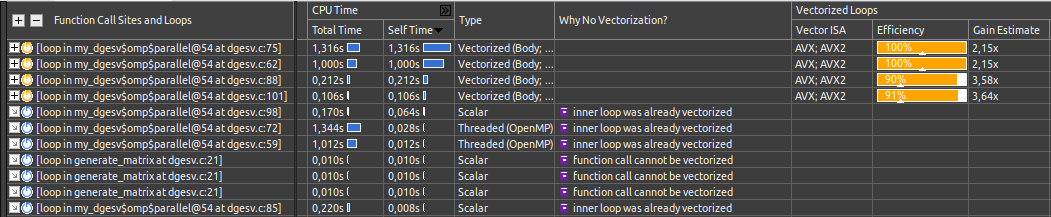
\includegraphics[width=0.95\textwidth]{img/gains_advisor.png}
	\caption{Datos de rendimiento de los bucles vectorizados relevantes}
	\label{fig:advisor_bucles}
\end{figure}
\begin{figure}[h]
	\centering
	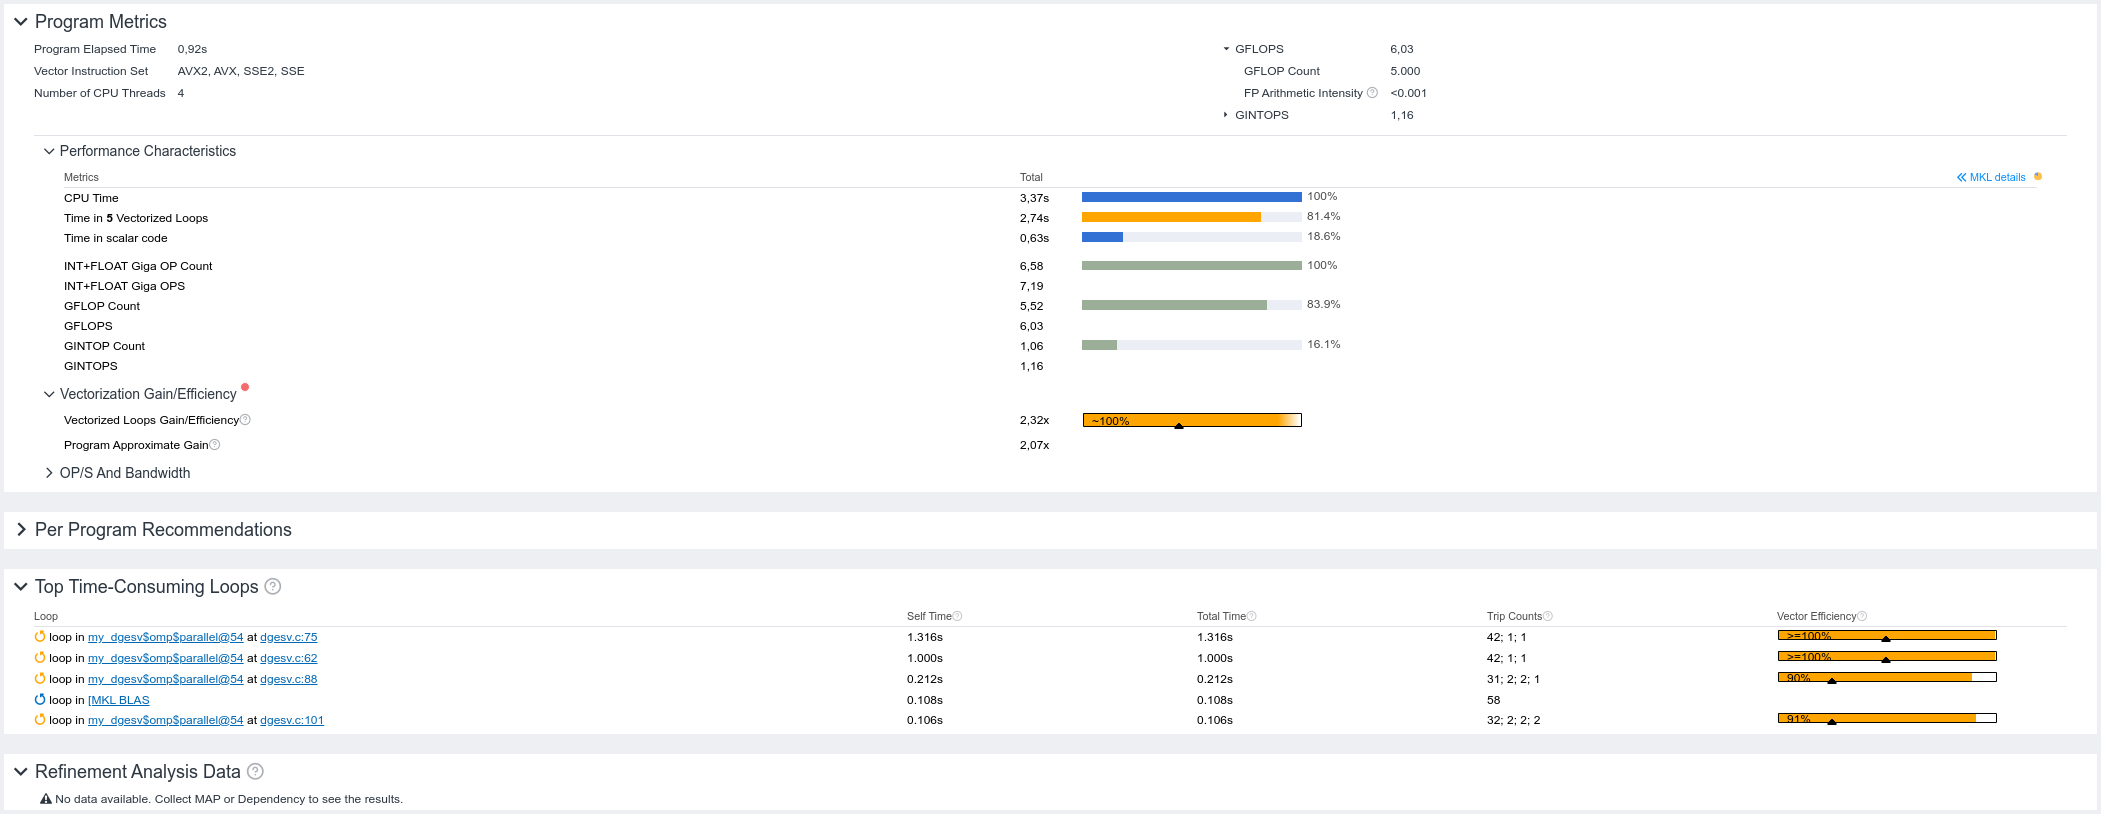
\includegraphics[width=\textwidth]{img/program_metrics.png}
	\caption{Métricas del programa completo, compilado con ICC}
	\label{fig:metricas}
\end{figure}
\begin{figure}[h]
	\centering
	\includegraphics[width=\textwidth]{img/µpipe_program.png}
	\caption{Datos de utilización de la arquitectura para el programa completo}
	\label{fig:micropipe}
\end{figure}
\end{document}
